% ============================================================================
%  sections/chapitre4.tex
% ============================================================================
\chapter{Implémentation, Asynchronisme et Tests}
\label{chapitre-4-implementation-asynchronisme-et-tests}

\section{Introduction}
Ce chapitre présente les aspects concrets de l'implémentation : les interfaces développées, la gestion de l'asynchronisme pour les opérations coûteuses, le système de notifications en temps réel, la sécurité et la stratégie de tests.

\section{Interfaces développées}
L'application comprend 11 interfaces principales, couvrant les trois rôles d'utilisateurs (Candidat, Responsable, Administrateur) :

\begin{table}[htbp]
\centering
\caption{Interfaces développées par rôle}
\label{tab:interfaces}
\begin{tabular}{p{4.5cm} p{2.5cm} p{7cm}}
\toprule
\textbf{Interface} & \textbf{Rôle} & \textbf{Description} \\
\midrule
Page d'accueil & Public & Landing page avec statistiques ENSA BM et filières \\
Authentification & Public & Inscription (email + CIN) et connexion JWT \\
Formulaire candidature & Candidat & 5 étapes avec sauvegarde brouillon \\
Suivi de dossier & Candidat & Statut temps réel avec badges colorés \\
Résultats épreuve & Candidat & Note, rang et résultat (Admis/Recalé) \\
Dashboard responsable & Responsable & KPIs, graphiques Recharts, actions \\
Gestion des dossiers & Responsable & Liste paginée, filtres, tri par score \\
Détail dossier & Responsable & Vue complète avec historique et alertes \\
Configuration admin & Admin & Filières, règles, pondérations \\
Import Excel & Responsable & Wizard 3 étapes avec mapping colonnes \\
Notifications & Tous & Cloche, panneau déroulant, historique \\
\bottomrule
\end{tabular}
\end{table}

\begin{figure}[htbp]
\centering
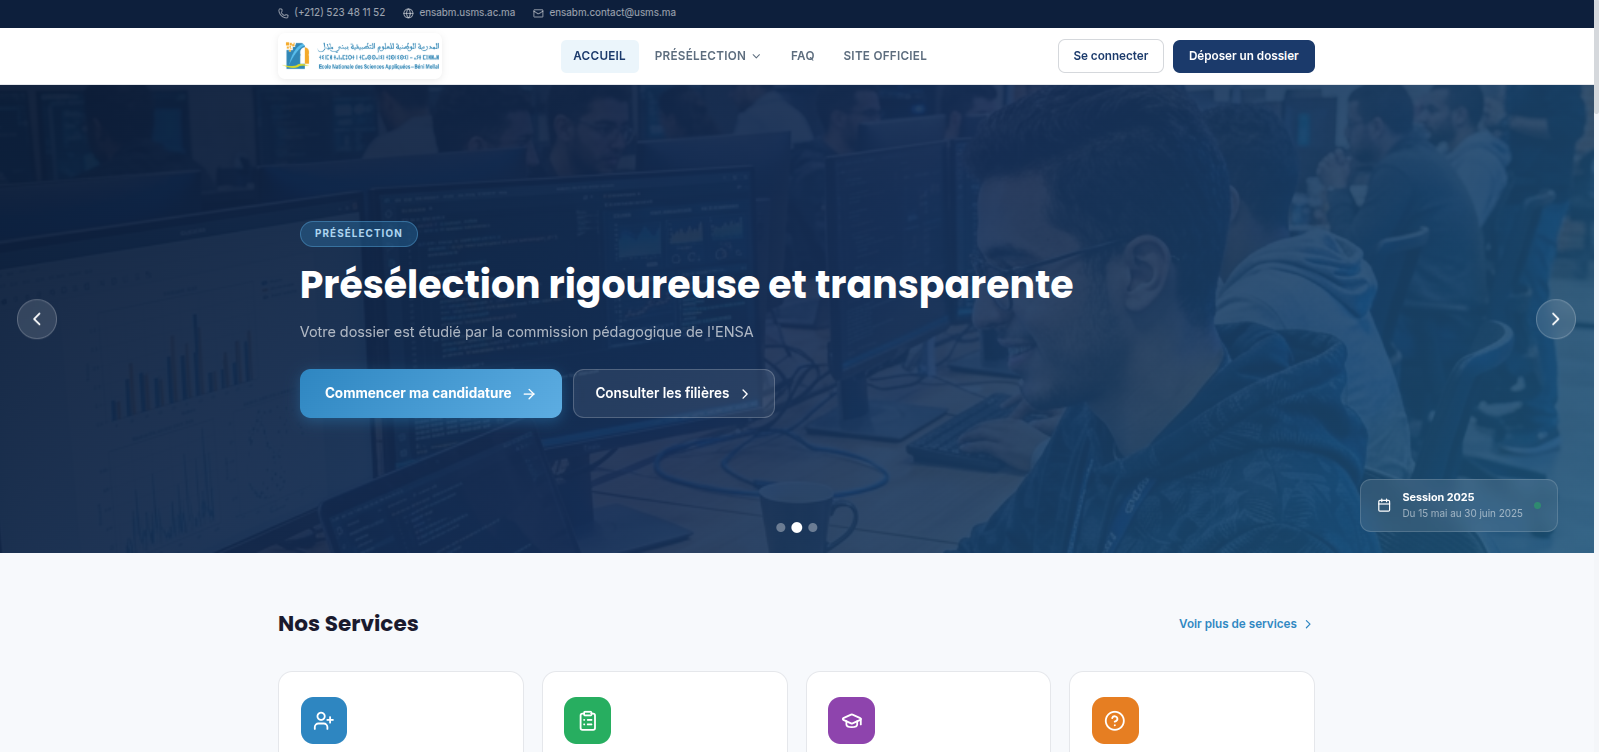
\includegraphics[width=0.85\textwidth]{media/image17.png}
\caption{Interface d'accueil de la plateforme}
\label{fig:interface-accueil}
\end{figure}

\begin{figure}[htbp]
\centering
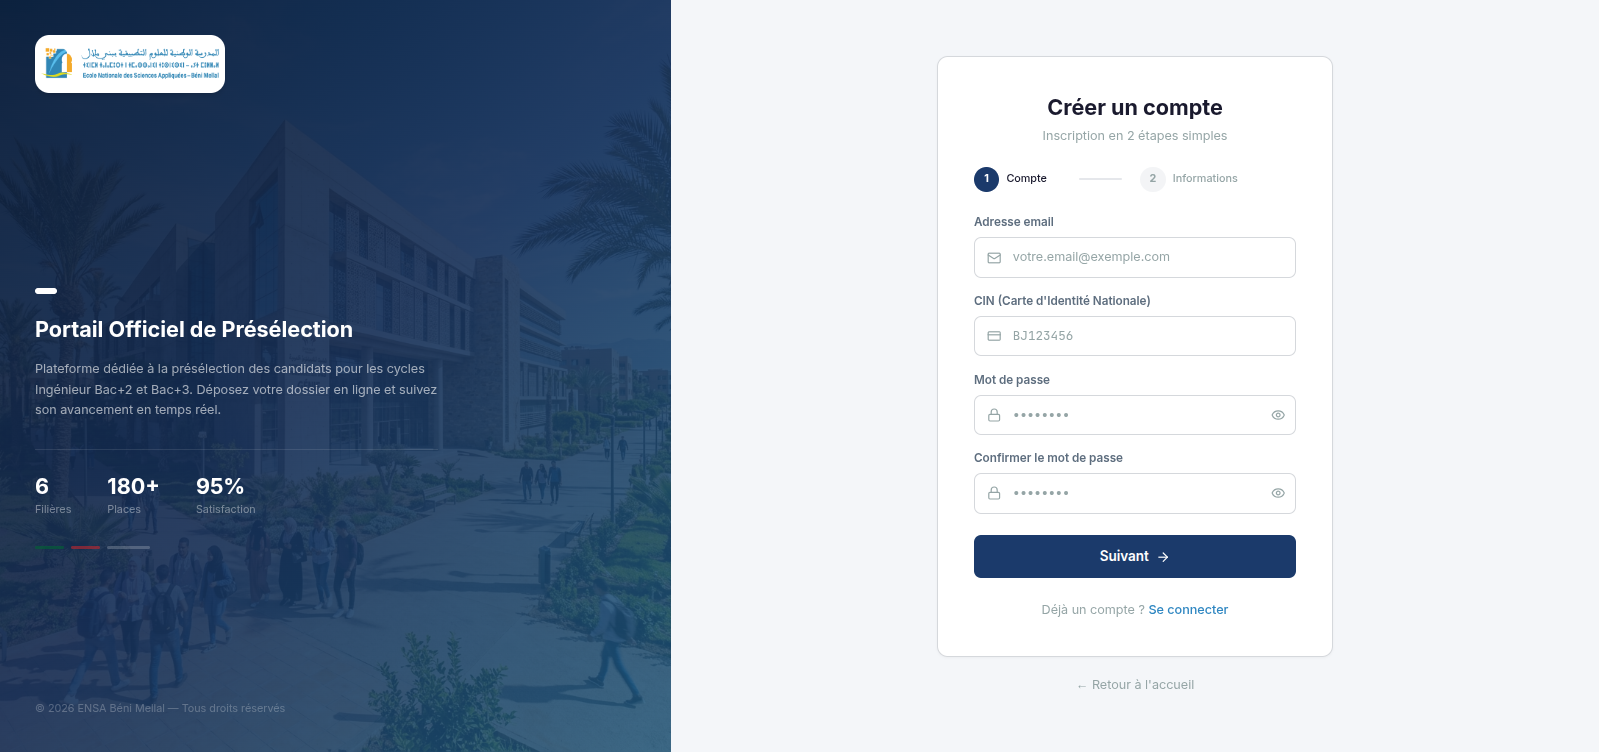
\includegraphics[width=0.85\textwidth]{media/image18.png}
\caption{Formulaire candidature}
\label{fig:formulaire}
\end{figure}

\begin{figure}[htbp]
\centering
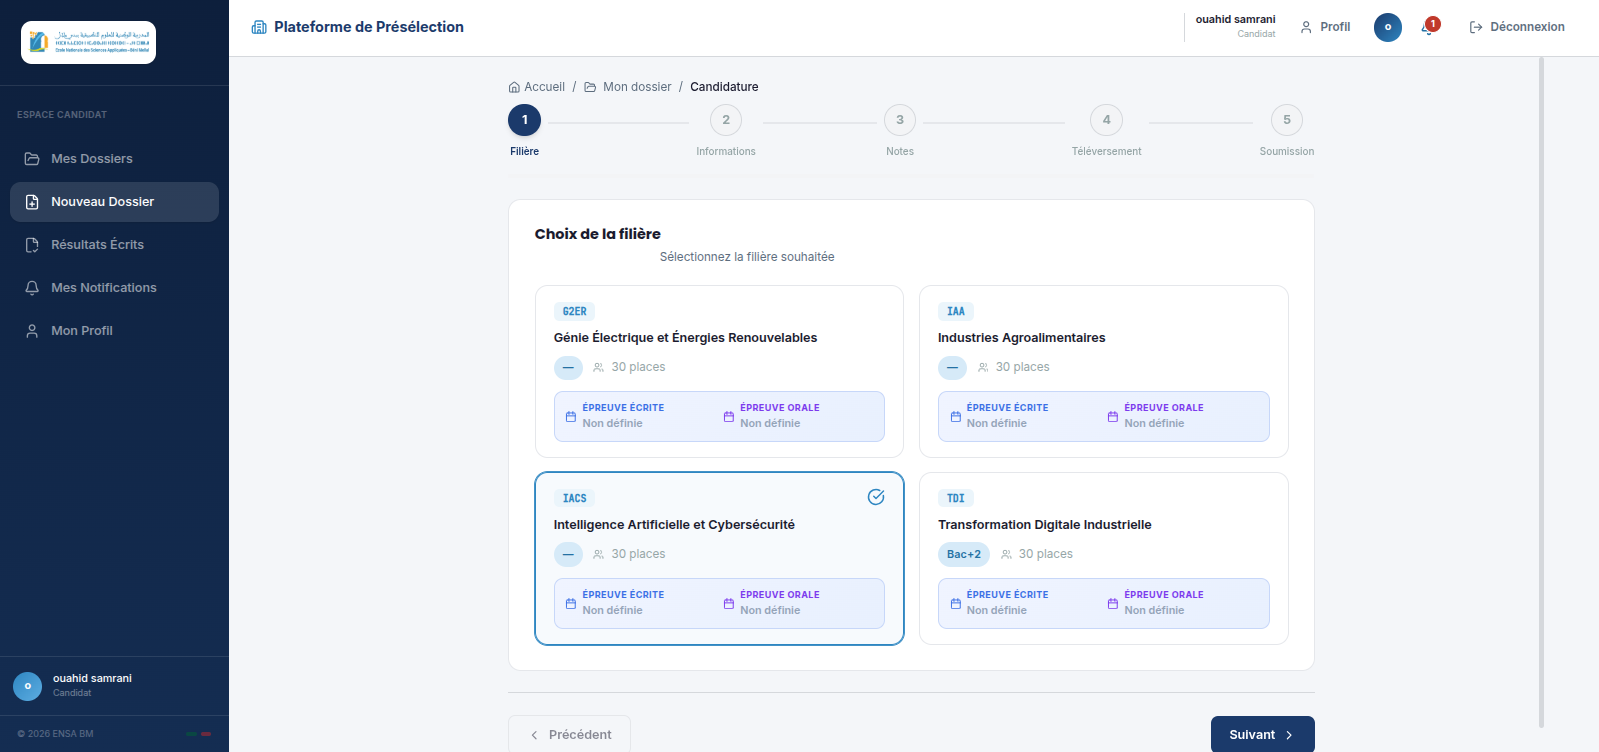
\includegraphics[width=0.85\textwidth]{media/image19.png}
\caption{Interface de dépôt des documents justificatifs}
\label{fig:documents}
\end{figure}

\begin{figure}[htbp]
\centering
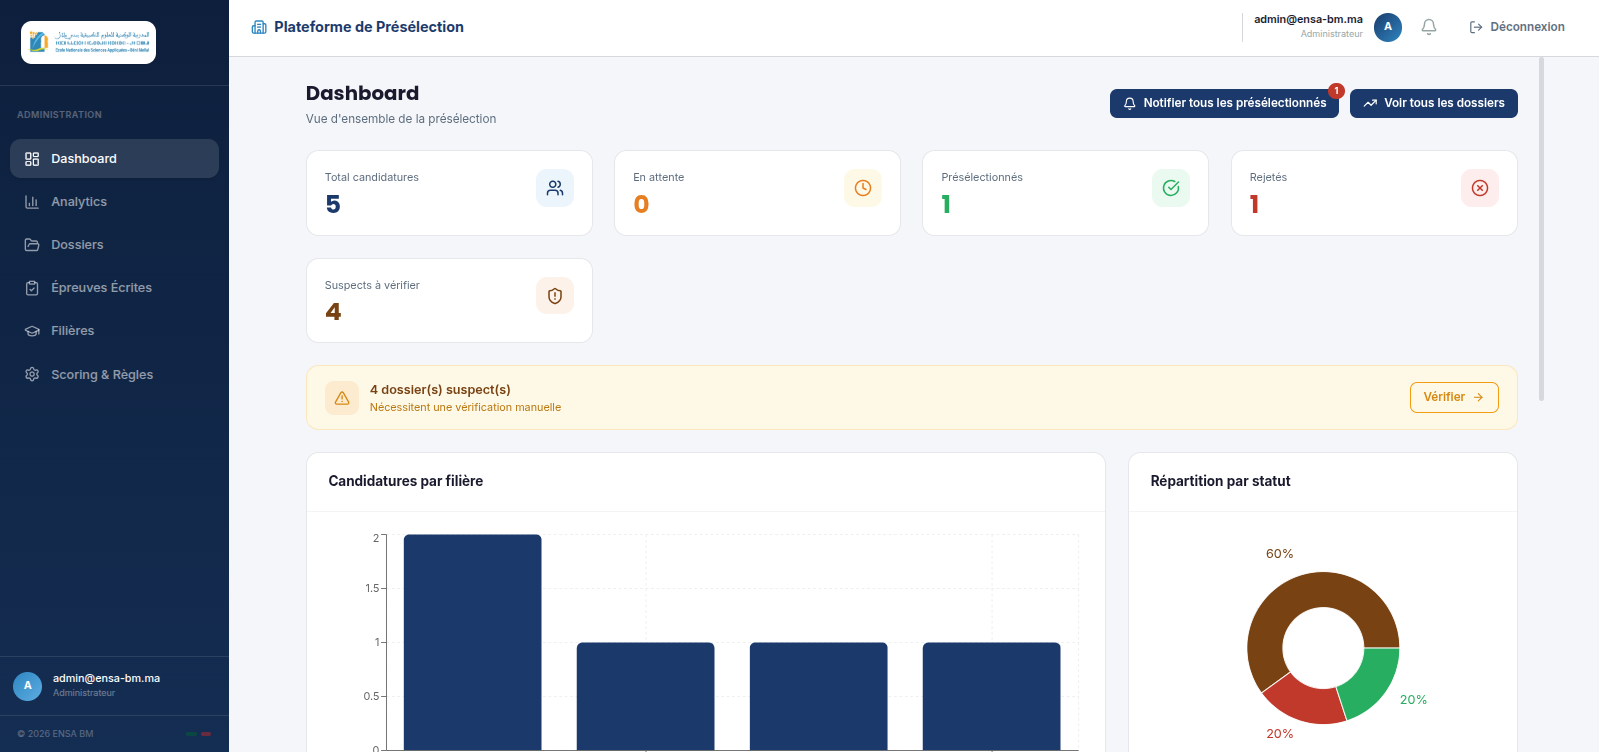
\includegraphics[width=0.85\textwidth]{media/image20.png}
\caption{Tableau de bord du responsable de présélection}
\label{fig:dashboard}
\end{figure}

\begin{figure}[htbp]
\centering
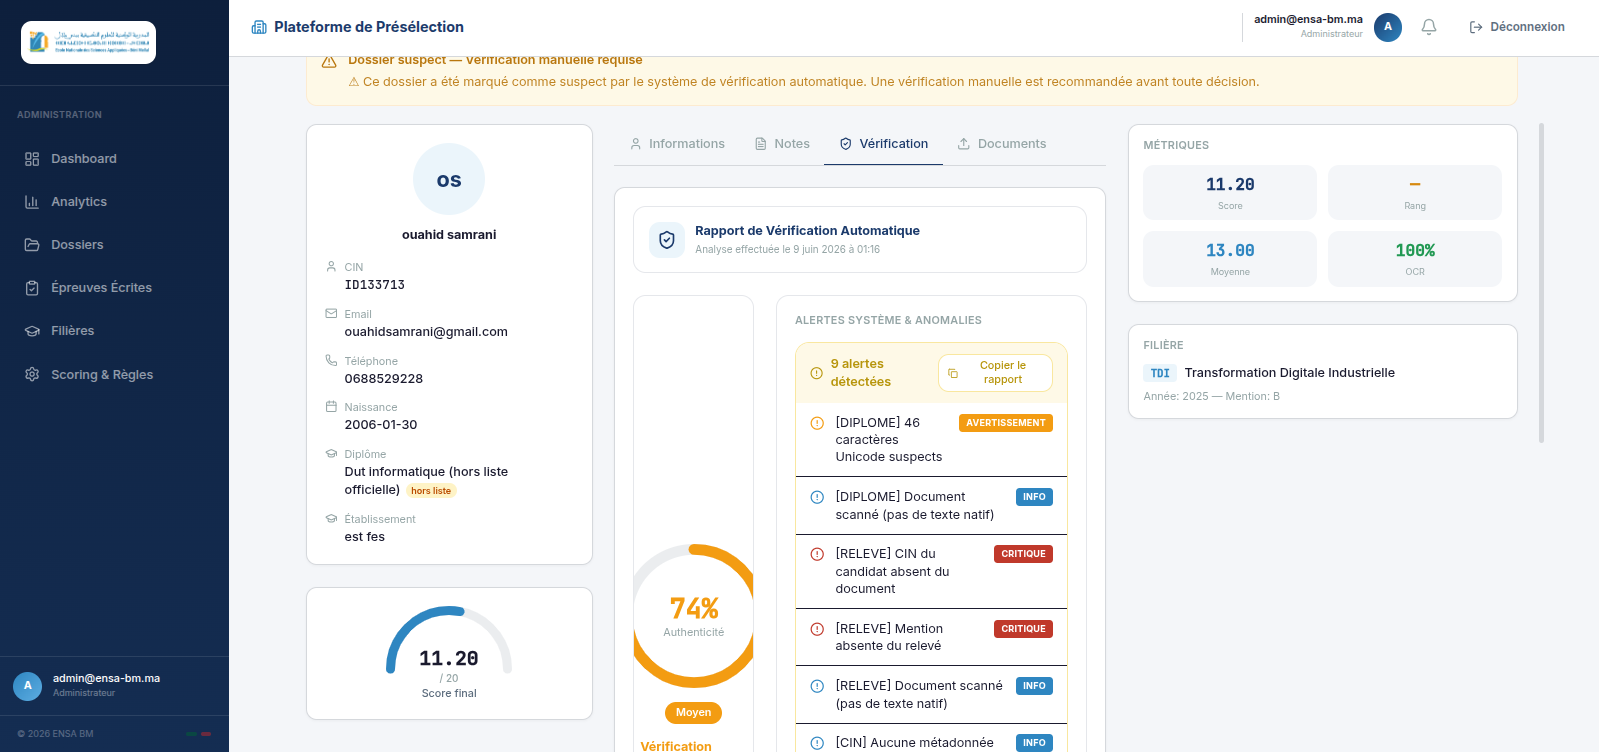
\includegraphics[width=0.85\textwidth]{media/image21.png}
\caption{Consultation détaillée d'un dossier candidat}
\label{fig:detail-dossier}
\end{figure}

\begin{figure}[htbp]
\centering
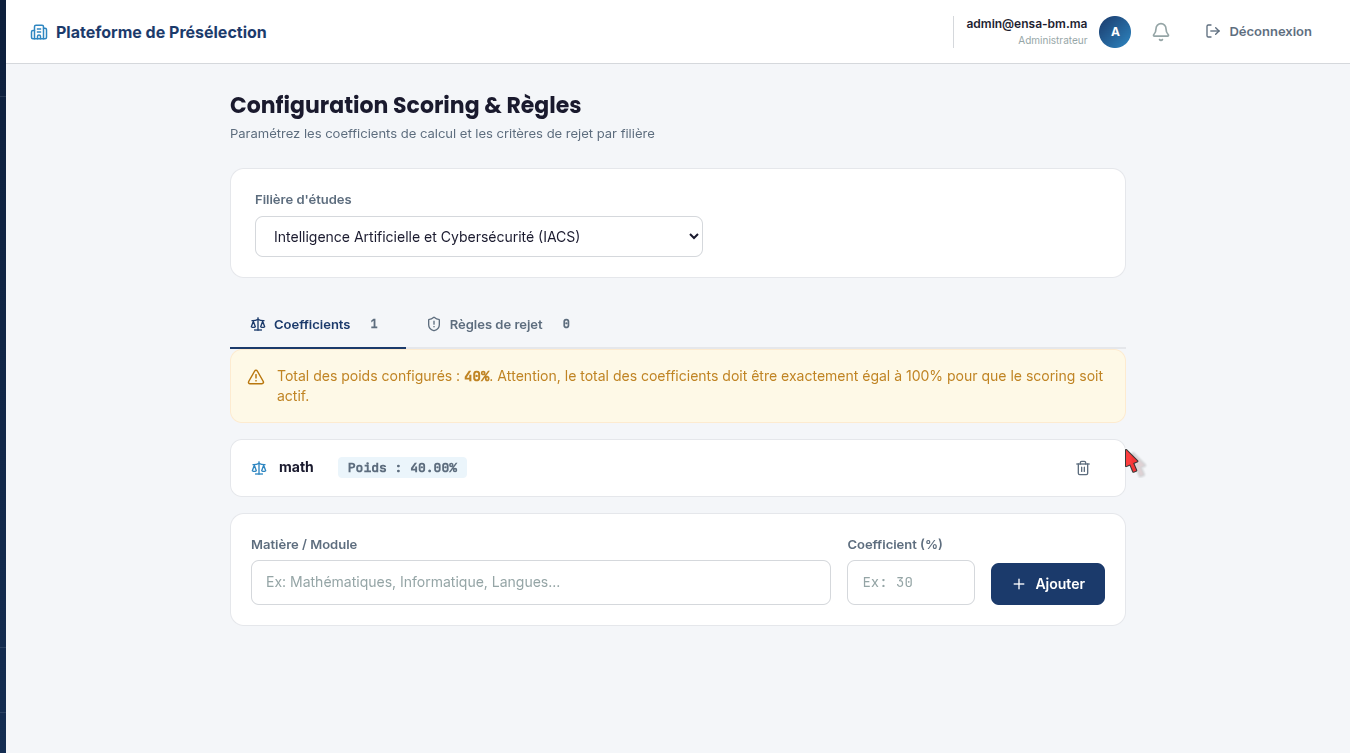
\includegraphics[width=0.85\textwidth]{media/image22.png}
\caption{Configuration des filières et règles de scoring}
\label{fig:config}
\end{figure}

\begin{figure}[htbp]
\centering
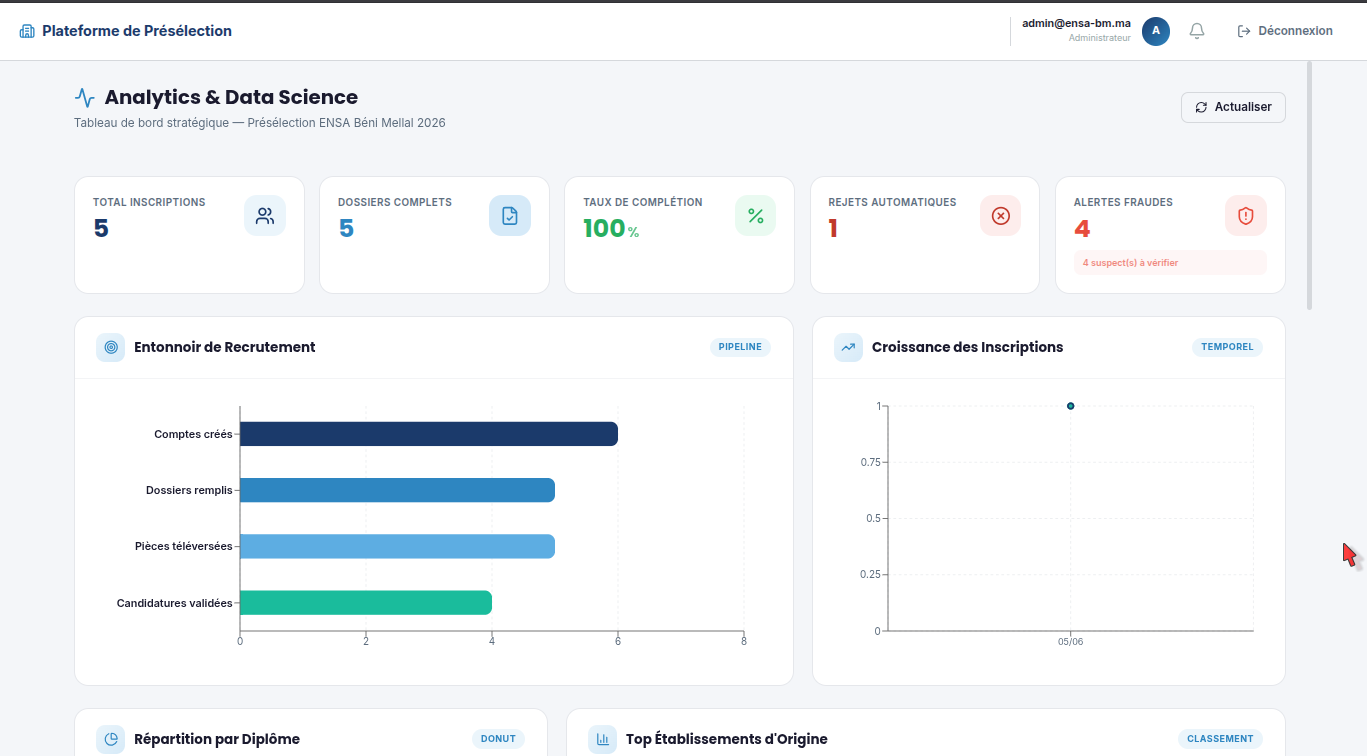
\includegraphics[width=0.85\textwidth]{media/image23.png}
\caption{Tableau de bord analytique du responsable de présélection}
\label{fig:analytics}
\end{figure}

\section{Gestion de l'asynchronisme}
\subsection{Problématique}
Plusieurs opérations de la plateforme sont coûteuses en temps d'exécution : le traitement OCR des documents, le calcul des scores, l'envoi d'emails en masse. Un traitement synchrone bloquerait l'interface utilisateur pendant plusieurs secondes.

\subsection{Solution : threading.Thread}
Pour garantir une excellente expérience utilisateur, l'application utilise l'asynchronisme via \texttt{threading.Thread} de Python. Les processus lourds sont exécutés en arrière-plan dans des threads démons. Le flux est le suivant :
\begin{itemize}
\item Le candidat soumet son dossier $\rightarrow$ réponse HTTP 200 immédiate
\item Un thread démon est lancé pour le traitement OCR et le scoring
\item Le thread ferme correctement sa connexion à la base de données après exécution
\item Le candidat est redirigé instantanément vers son dashboard
\item Le statut du dossier est mis à jour en arrière-plan et notifié via WebSocket
\end{itemize}

\subsection{Gestion des connexions base de données}
Le système veille à clore correctement les connexions à la base de données dans les threads via \texttt{django.db.connections.close\_all()} pour éviter toute fuite de connexion ou conflit d'accès concurrent.

\section{Système de notifications en temps réel}
\subsection{Architecture WebSocket}
Les notifications combinent deux canaux complémentaires :
\begin{itemize}
\item SMTP (Gmail App Password) : envoi d'emails avec gestion des erreurs et statut persisté
\item Django Channels + Redis : notifications WebSocket temps réel avec barre de progression pour les envois en masse
\end{itemize}

\subsection{Envoi en masse avec progression}
Lors de l'envoi de notifications en masse, le backend envoie les emails par batch SMTP et notifie le frontend de la progression en temps réel via WebSocket. Le responsable voit une barre de progression se remplir au fur et à mesure des envois.

\section{Système de logging}
L'application intègre un mécanisme de traçabilité sécurisé par fichiers. La configuration Django dirige les flux vers un fichier central (logs/ensa\_presel.log). Les logs sont structurés par domaine :

\begin{table}[htbp]
\centering
\caption{Configuration des loggers}
\label{tab:loggers}
\begin{tabular}{p{3cm} p{3cm} p{8cm}}
\toprule
\textbf{Logger} & \textbf{Niveau} & \textbf{Usage} \\
\midrule
django & WARNING & Erreurs framework \\
candidatures & INFO & Opérations métier \\
notifications & INFO & Envois email/WebSocket \\
channels & DEBUG & Connexions WebSocket \\
\bottomrule
\end{tabular}
\end{table}

\section{Sécurité de l'application}
\begin{table}[htbp]
\centering
\caption{Mesures de sécurité implémentées}
\label{tab:securite}
\begin{tabular}{p{4cm} p{10cm}}
\toprule
\textbf{Mesure} & \textbf{Implémentation} \\
\midrule
Authentification & JWT (access 15min + refresh 24h) \\
Autorisation & RBAC à 3 niveaux via @permission\_classes \\
CSRF & Protection Django middleware activée \\
XSS & Échappement automatique Django + React \\
Injection SQL & ORM Django avec requêtes paramétrées \\
Logs sécurisés & Fichier avec rotation, pas de console \\
Confidentialité & Scores OCR masqués côté candidat \\
\bottomrule
\end{tabular}
\end{table}

\section{Stratégie de tests}
\subsection{Niveaux de tests}
\begin{table}[htbp]
\centering
\caption{Niveaux de tests}
\label{tab:niveaux-tests}
\begin{tabular}{p{3.5cm} p{7cm} p{4cm}}
\toprule
\textbf{Niveau} & \textbf{Objectif} & \textbf{Outils} \\
\midrule
Tests unitaires & Valider chaque composant isolément & Django TestCase \\
Tests d'intégration & Valider les flux complets & APITestCase, APIClient \\
Tests fonctionnels & Valider les scénarios utilisateur & Scénarios manuels \\
Tests d'interface & Valider le responsive et l'UX & Navigateur, DevTools \\
\bottomrule
\end{tabular}
\end{table}

\subsection{Tests du moteur de règles}
\begin{table}[htbp]
\centering
\caption{Tests du moteur de règles}
\label{tab:tests-regles}
\begin{tabular}{p{3.5cm} p{4.5cm} p{3.5cm} p{2.5cm}}
\toprule
\textbf{Test} & \textbf{Entrée} & \textbf{Résultat attendu} & \textbf{Statut} \\
\midrule
Diplôme invalide & DUT non accepté pour TDI & REJETE\_AUTO & $\checkmark$ Passé \\
Moyenne insuffisante & Moyenne 9.5 (seuil 10) & REJETE\_AUTO & $\checkmark$ Passé \\
Doublon CIN & CIN déjà existant & REJETE\_AUTO & $\checkmark$ Passé \\
Dossier conforme & Tous critères OK & EN\_ATTENTE & $\checkmark$ Passé \\
\bottomrule
\end{tabular}
\end{table}

\subsection{Tests de l'algorithme de scoring}
\begin{table}[htbp]
\centering
\caption{Tests de l'algorithme de scoring}
\label{tab:tests-scoring}
\begin{tabular}{p{3.5cm} p{4.5cm} p{3cm} p{2.5cm}}
\toprule
\textbf{Test} & \textbf{Données} & \textbf{Score attendu} & \textbf{Statut} \\
\midrule
Scoring TDI & Moyennes S1-S6, DUT Info & 15.42 & $\checkmark$ Passé \\
Scoring IACS & Moyennes S1-S6, Licence Info & 14.87 & $\checkmark$ Passé \\
Bonus mention TB & Moyenne $\geq$16 & +2.0 bonus & $\checkmark$ Passé \\
\bottomrule
\end{tabular}
\end{table}

\subsection{Récapitulatif des tests}
\begin{table}[htbp]
\centering
\caption{Récapitulatif des résultats de tests}
\label{tab:recap-tests}
\begin{tabular}{p{4cm} p{2cm} p{2cm} p{2cm}}
\toprule
\textbf{Type de test} & \textbf{Nombre} & \textbf{Passés} & \textbf{Échoués} \\
\midrule
Unitaires & 32 & 32 & 0 \\
Intégration & 12 & 12 & 0 \\
Fonctionnels & 9 & 9 & 0 \\
Interface & 8 & 8 & 0 \\
\midrule
\textbf{Total} & \textbf{61} & \textbf{61} & \textbf{0} \\
\bottomrule
\end{tabular}
\end{table}

\subsection{Couverture de code}
\begin{table}[htbp]
\centering
\caption{Couverture de code par module}
\label{tab:couverture}
\begin{tabular}{p{4cm} p{3cm}}
\toprule
\textbf{Module} & \textbf{Couverture} \\
\midrule
users & 89\% \\
candidatures & 92\% \\
administration & 85\% \\
scoring & 94\% \\
notifications & 78\% \\
\midrule
\textbf{Global} & \textbf{87\%} \\
\bottomrule
\end{tabular}
\end{table}

\section{Difficultés rencontrées et solutions}
\begin{table}[htbp]
\centering
\caption{Difficultés rencontrées et solutions}
\label{tab:difficultes}
\begin{tabular}{p{5cm} p{9cm}}
\toprule
\textbf{Difficulté} & \textbf{Solution apportée} \\
\midrule
WebSocket + JWT expiré & Middleware WebSocket avec refresh automatique du token \\
SMTP Gmail bloqué & Configuration App Password avec gestion des erreurs \\
Imports circulaires Django & Import local dans les méthodes au lieu d'imports globaux \\
OCR faible qualité & Fallback sur moyenne générale + flag SUSPECT \\
Connexions DB dans threads & Appel systématique à \texttt{connections.close\_all()} \\
\bottomrule
\end{tabular}
\end{table}

\section{Conclusion}
Ce chapitre a présenté les aspects concrets de l'implémentation : les 11 interfaces développées, la gestion de l'asynchronisme via threading, le système de notifications WebSocket temps réel, la sécurité robuste et la stratégie de tests complète avec un taux de réussite de 100\% et une couverture de code de 87\%.
